\documentclass{article}

\usepackage{graphicx}
\usepackage{amssymb, amsmath}
\usepackage{bm} % more powerful version to get bold

\usepackage{xcolor}

\usepackage[backend=biber, style=apa,autocite=inline]{biblatex} % package for bibliography
\DeclareLanguageMapping{english}{english-apa}

\addbibresource{sdewind.bib}

%\usepackage[backend=biber, style=authoryear,autocite=inline]{biblatex}

\newcommand{\add}{\textcolor{red}{[insert]}}

\setcounter{page}{1}

\begin{document}

\title{ Stochastic Wind Power Forecasting }  % \\  \small{Report}}

\author{ Waled Alhaddad\textsuperscript{\textasteriskcentered} \qquad Ahmed Kebaier\textsuperscript{\ddag} \qquad Ra\'ul  Tempone\textsuperscript{\textasteriskcentered}\textsuperscript{\textdagger} \\
\textsuperscript{\textasteriskcentered}CEMSE Division, King Abdullah University of Science and Technology (KAUST), Saudi Arabia \\ \textsuperscript{\textdagger}Alexander von Humboldt Professor, RWTH Aachen University,  Germany
 \\ \textsuperscript{\ddag}Université Paris 13, Sorbonne Paris Cité, LAGA, CNRS (UMR 7539) , Villetaneuse , France }

\maketitle
%\thispagestyle{empty}
{\color{red}Keywords: Indirect inference, wind power, probabilistic forecasting, stochastic differential equations, Lamperti transform, model selection, sensitivity.}
%%%%%%%%% ABSTRACT

\begin{abstract}

Reliable wind power generation forecasting is crucial for applications such as the allocation of energy reserves, optimization of electricity price and operation scheduling of conventional power plant. We propose a data driven model based on parametric Stochastic Differential Equations (SDEs) to captures real-world asymmetric dynamics of wind power forecast errors. Our SDE framework incorporates time derivative tracking of the forecast, time-dependent mean reversion parameter and an improved diffusion term. We are able to simulate future wind power production paths and to get sharp confidence bands. The method is forecast technology agnostic and enables the comparison between different forecasting technologies on the basis of information criteria. We apply the model to historical French and Uruguayan wind power production data and forecasts on the period (2017-2018).

\end{abstract}

%%%%%%%%% BODY TEXT


%---BEGIN SECTION 1---
\section{Introduction}  \label{Section_1}

Reliable wind power generation forecasting is crucial for the following applications [ref]:
\begin{itemize}
\item Allocation of energy reserves such as water levels in dams or oil, and gas reserves.
\item Operation scheduling of non-controlable power plants.
\item Optimization of the price of electricity for different parties such as electric utilities, Transmission system operator (TSOs), Electricity service providers (ESPs), Independent power producers (IPPs), and energy traders.
\item Maintenance planning such as that of power plants components and transmission lines.

\end{itemize}

Different methods have been applied to wind power forecasting. They can be generally categorized as follows: physical models, statistical methods, artificial intelligence methods and hybrid approaches. The output of such methods is usually a deterministic forecast. Occasionally probabilistic forecasts are produced through uncertainty propagation in the data, parameters or through forecast ensembles. However, there is a lacking in simulating and producing data driven stochastic forecasts based on real-world performance of forecasting models. It is crucial to capture actual performance of a forecast as it has been known that different forecasting technologies exhibits different behavior for different wind farms and seasons [ref]. This is due to many factors which forecast are challenged to capture such as the surrounding terrains of the wind farm and the condition of the blades such as icing, wear and tear or dirt. It is known that complex terrains in both off shore and on shore locations decrease the accuracy of wind power forecasts significantly [ref]. It also has been shown that the performance of forecasts varies from month to month. Thus the performance of wind power forecasts is location and time dependent.

Many approaches have been taken to evaluate the uncertainty of a given forecast. There are two types of errors: level errors and phase errors. The use of mean or median errors in this context may be misleading as wind power forecast errors are asymmetric. This is a natural consequence of wind power being non-negative and bounded by the maximuim capacity of production. This is important as the associated cost to power forecast errors are also asymmetric due to different costs for up and down  power regulations which are determined by the electricity market [ref].

We propose to model wind power forecasts errors using parametric stochastic differential equations (SDEs) whose solution defines a stochastic process. This resultant stochastic process describes the time evolution dynamics of wind power forecast errors while capturing properties such as a correlation structure and the inherent asymmetry. Additionally, the model we propose is agnostic of the forecasting technology and serves to complement forecasting procedures by providing a data driven stochastic forecast. Hence, we are able to evaluate wind power forecasts according to their real-world performance and we are able to compare different forecasting technologies. Most notably, we are able to simulate future wind power production given a deterministic wind power forecast. Future wind power production using Monte Carlo methods, as well as the analytic form of the proposed SDE, can be used in optimal control problems involving wind power production.

Previous attempt by (\cite{mozuma}) considered stochastic wind power forecast models based on stochastic differential equations (SDEs). Here, we propose an improved model featuring time derivative tracking of the forecast, time-dependent mean reversion, modified diffusion and non-Gaussian approximations. We apply the model to French and Uruguayan wind power forecasts together with historical wind power production data pertaining to the year 2017-2018.

We use a year long data set from Uruguay based on 1000 observation paths, each of which is 72-hours long with observations recorded every 10 min. In total, it is a data set of approximatly half a million data points recorded in 2018. See Figure (\ref{fig:sample_data}). The data is normalized with respect to the maximuim power capacity of wind power production in Uruguay. The asymmetry or skew nature of the data is clear when inspected for different power production levels. We split the aggregated data into a low, meduim and high power range. See Figure (\ref{fig:skew_data}).

In this paper we present the phenomenological underlying model in Section \ref{Section_2} and describe the physical constraints in Section \ref{Section_3} and how these constrains can be met. Then, in Section \ref{Section_4}, we will introduce an alternative formulation of the model in Lamperti space. In Section \ref{Section_5}, we show our parameter estimation procedure and its results in Section \ref{Section_6}. We compare alternative models in Section \ref{Section_7} and different forecast providers in Section \ref{Section_8}.

\begin{figure}
  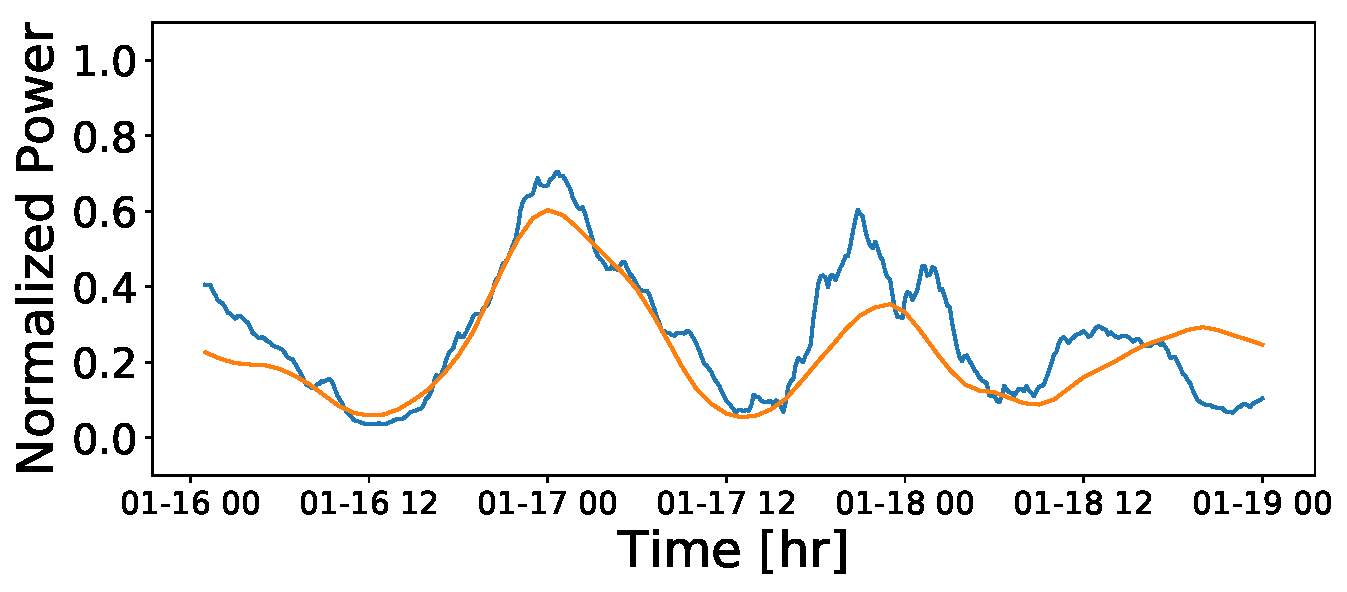
\includegraphics[width=60mm,scale=1]{plots/data_1516064400.pdf}
  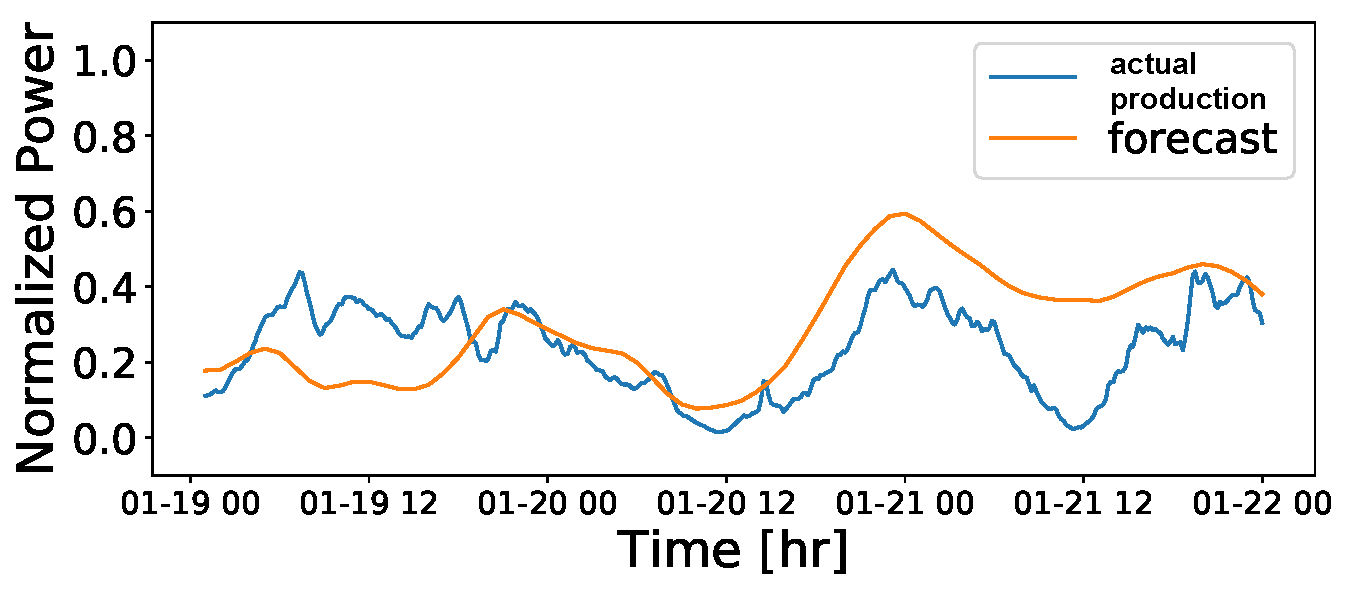
\includegraphics[width=60mm,scale=1]{plots/data_1516323600.pdf}\\
  \caption{Two samples from the Uruguayan of 2018. Each sample compromises of two 72-hour paths. In yellow is an hourly wind power production forecast. In blue is the actual wind power production recorded in 10 minute intervals.}
  \label{fig:sample_data}
\end{figure}

\begin{figure}
  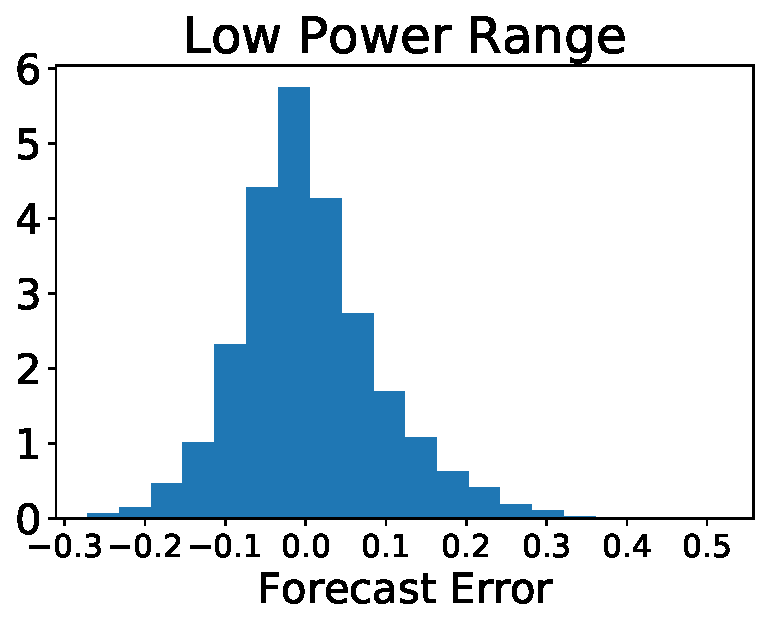
\includegraphics[width=38mm,scale=1]{plots/hist_low.pdf}
  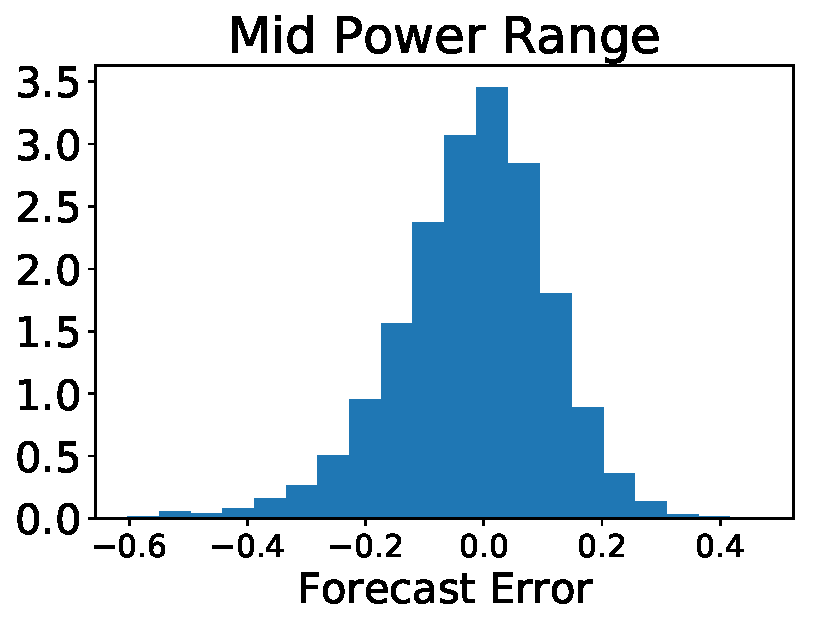
\includegraphics[width=38mm,scale=1]{plots/hist_mid.pdf}
  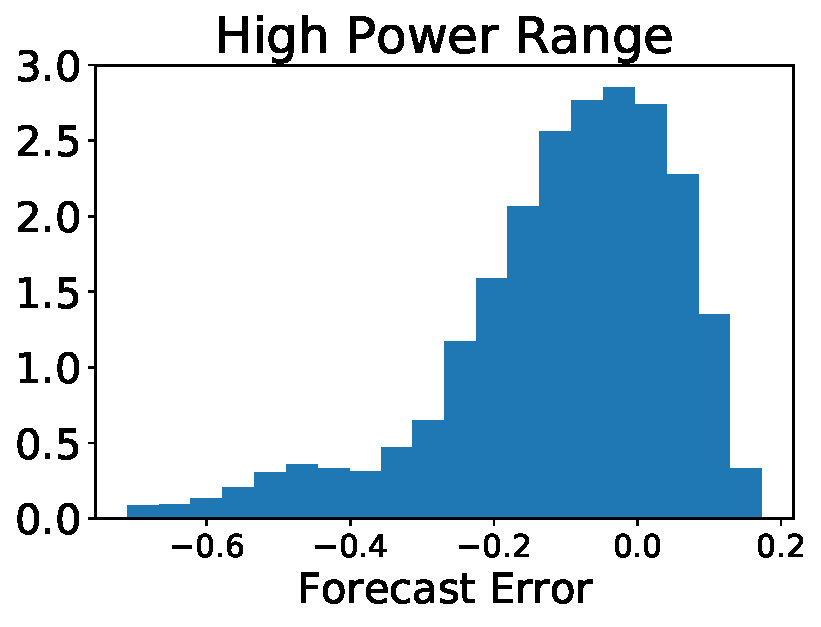
\includegraphics[width=38mm,scale=1]{plots/hist_high.pdf}
  \caption{We see that forecast errors exhibit skewness near the boundries (i.e. low and high power production regimes.). Low power is when produced power is less than $0.3$, mid power is when it is between $0.3$ and $0.6$ and high power when is larger than $0.6$. }
  \label{fig:skew_data}
\end{figure}

\begin{figure}
  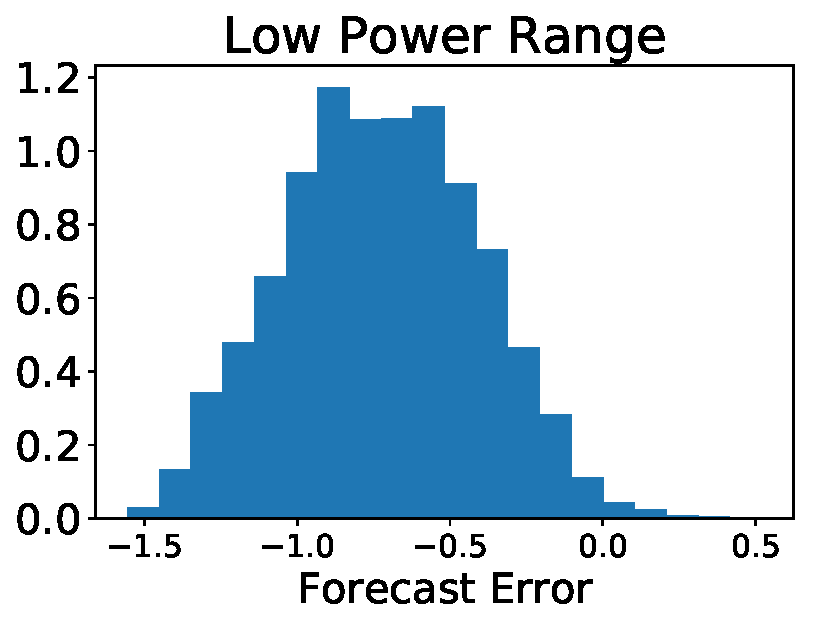
\includegraphics[width=38mm,scale=1]{plots/hist_low_lamperti.pdf}
  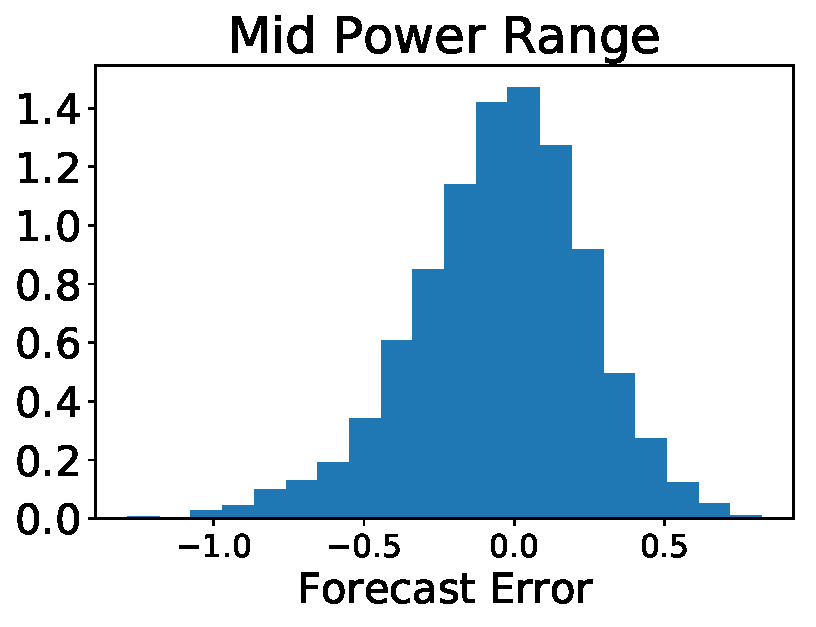
\includegraphics[width=38mm,scale=1]{plots/hist_mid_lamperti.pdf}
  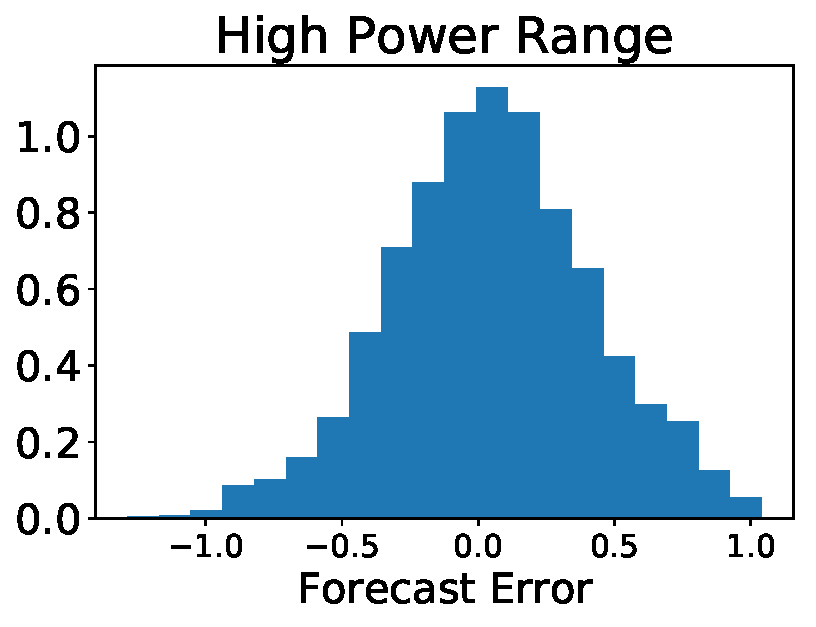
\includegraphics[width=38mm,scale=1]{plots/hist_high_lamperti.pdf}
  \caption{We observe that skewness has been greatly reduced after the Lamperti transformation. This motivates us to use a Gaussian transition density as a proxy density.}
  \label{fig:skew_after_lamperti}
\end{figure}
%---END SECTION 1---

%---BEGIN SECTION 2---
\section{Phenomenological  Model} \label{Section_2}

We introduce the following phenomenological model. Let $\{X_t, \, t>0\}$  be the  wind power generation forecasts stochastic process defined by the following parameterized stochastic differential equation (SDE)

\begin{align}
dX_t & =  a(X_t; p_t, \dot{p}_t,\bm{\theta}) \ dt + b (X_t; p_t, \bm{\theta} ) \ dW_t \nonumber \\ 
X_0 & =  x_0\,,   \label{eq:main}
\end{align}
where


\begin{itemize}
\item $a(\cdot; p_t, \dot{p}_t,\bm{\theta}):[0,1] \to \mathbb{R} \ $  denotes a drift function,
\item $b (\cdot;p_t, \bm{\theta} ):[0,1] \to \mathbb{R} \ $  a  diffusion function,
\item $\bm{\theta}$ is a vector of parameters,
\item $p_t$ is a time-dependent scalar value and $ \dot{p}_t$ is its time derivative at time $t$,
\item $\{W_t, \, t >0\}$ is a standard Wiener process in $\mathbb{R}$.
\end{itemize}

 In this work, $p_t$ is to be considered as a deterministic forecast of the wind power generation at time $t$ which is available from an official source. 

Our goal is to provide a specification of the model (\ref{eq:main}) to follow closely the available wind power forecasts while ensuring its unbiasedness with respect to the forecast. It is straightforward to show that $\mathbb{E} \left[X_t\right] = p_t$, where $p_t$ is the available deterministic wind power forecast for the time $t$.

\subsection{Physical Constrains}

Let $p_t$ be a numerical wind power forecast, which is an input to this approach. Assume that the wind power generation forecasts are modeled as solutions to the following It\^{o} stochastic differential equation
\begin{align}
dX_t&= \dot{p}_t \ dt - \theta_t (X_t - p_t) \ dt + b (X_t; \bm{\theta} ) \ dW_t\,, \quad t > 0 \nonumber \\
X_0 &= x_0\,. \label{model:derivative_tracking_X}
\end{align}

According to the SDE specification in (\ref{model:derivative_tracking_X}), the process $X_t$ satisfies the two following properties: \begin{itemize}
\item it is mean reverting to the wind power forecast $p_t$, and 
\item it tracks the time derivative wind power forecast $\dot{p}_t$.  
\end{itemize} 
Observe that a mean reverting model without derivative tracking exhibits consistent lags, as it is shown in Figure (\ref{fig:derivative_tracking}). See Section \ref{Section_7} for comparisons.

\begin{figure}
  %\includegraphics[width=26mm,scale=1]{}
  \caption{insert figure showing the difference with and without derivative tracking}
  \label{fig:derivative_tracking}
\end{figure}


We normalize the forecast and production data to Uruguay  installed power capacity at the time of observation. Thus our process must be limited to the range $[0,1]$. To enforce this constraint, our  drift and diffusion terms  must satisfy certain rules.
 

Let $\bm{\theta} = (\theta_0,\alpha)$. We want a process that follow the wind forecast, thus we choose mean reverting drift term which also tracks the derivative of $p_t$, which is an input to our model.
  \begin{equation}
    a(x; p_t,\bm{\theta})=  \dot{p_t} - \theta_t(x - p_t)
  \end{equation}
where $\theta_t>0$ is a time-dependent parameter that controls the speed of reversion.


We would like  a diffusion term that vanishes at the boundaries to prevent the process from escaping the region $[0,1]$.
  \begin{equation}
    b (x; p_t,\bm{\theta} )= \sqrt{2 \theta_t \alpha x (1-x)}
  \end{equation}
  where $\alpha >0$ is a constant parameter that controls the path variability. This diffusion term belongs to the Pearson diffusion family and , in particular, it is a Jacobi type diffusion.

To further ensure that the process does not escape the region $[0,1]$, the mean reversion parameter has to be selected according to the following rule. Observe that the time derivative term $\dot{p}_t $ is not controlled to maintain that $X_t$ stays a.s.  inside the range $[0,1]$. In other words, the zero drift line defined by $a(x; p_t,\bm{\theta}) =0$, which an attractor, must be contained inside the range $[0,1]$. Thus, we must have that
\begin{equation}
\frac{- |\dot{p_t}|}{p_t} \leq \theta \leq \frac{|\dot{p}_t|}{1- p_t}
\end{equation}
which is satisfied  by choosing a time-dependent  $\theta_t$ as follows,
\begin{equation}
\theta_t = \max \left( \theta_0 \ , \ \frac{|\dot{p}_t|}{\min (p_t, 1-p_t)}  \right ),  \quad \theta_0 >0 \label{theta_t}
\end{equation}

\subsubsection*{Change of Variables:}
To avoid differentiation of the forecast $p_t$ and simplify, we apply the change of variables $$V_t = X_t - p_t \,.$$ 

The  model becomes,
\begin{align}
dV_t &=  - \theta_t V_t \  dt + \sqrt{2 \theta_t \alpha (V_t +p_t ) (1-V_t-p_t)} \  dW_t  \nonumber \\ %\quad t > 0
V_0 & = v_0 \,. \label{VtSDE}
% \theta_t &= \max \left( \theta_0 \ , \ \frac{|\dot{p}_t|}{\min (p_t, 1-p_t)}  \right )\\
\end{align}
%---END SECTION 2---


%---BEGIN SECTION 3---
\section{State independent diffusion: Lamperti transform} \label{Section_3}

Our model (\ref{VtSDE}) for the forecast error has a diffusion term that depends on the state variable $V_t$. To estimate the unknown model parameters, a recommended technique is to modify the SDE (\ref{VtSDE}) by applying the so-called Lamperti transform (see \cite[40--41]{iacus1}, \cite{moma}, \cite[98--100]{saso}) to the process $V$ to obtain a SDE for the transformed process whose diffusion term does not depend anymore on the state variable. \\

We consider the following transformation 
\begin{equation}
Z_t = h(V_t) = \int_{\xi}^{x} \frac{1}{\sqrt{(u + p_t)(1 - u - p_t)}} \,du \Bigg{\vert}_{x = V_t} \,,
\end{equation}
where $\xi$ is an arbitrary point of the state space of the process $V$. The choice of $\xi = \frac{1}{2} - p_t$, where $p_t$ is a known input, leads to the process 
\begin{equation}
Z_t = h(V_t) = \arcsin (2(V_t + p_t) -1)\,,
\end{equation}
that, after applying It\^{o}'s formula on $h(V_t)$, gives the state-independent diffusion SDE
\begin{equation}
dZ_t = \left[  \frac{- \theta_t V_t}{\sqrt{(V_t + p_t)(1 - V_t - p_t)}} - \frac{1}{2} \frac{\left( \frac{1}{2} - (V_t + p_t)\right)}{(V_t + p_t)(1 - V_t - p_t)}  \right] \,dt + \sqrt{2 \theta_t \alpha}\, dW_t \,. \label{eq:stindepSDE}
\end{equation}
After replacing $V_t = \frac{\sin(Z_t) + 1}{2} - p_t$ in (\ref{eq:stindepSDE}), we obtain that the  process $Z$ satisfies the SDE
\begin{equation}
dZ_t = \frac{- \theta_t (\sin(Z_t) + 1 - 2 p_t) + \frac{\sin{Z_t}}{2}}{\cos{Z_t}} \,dt + \sqrt{2 \theta_t \alpha}\, dW_t \,. \label{eq:stindepSDE}
\end{equation}


%\begin{align}
%    dZ_t&= \frac{- \theta_t (1+ \sin(Z_t) - 2p_t) + \alpha \theta_t \sin (Z_t)   }{\cos (Z_t)} \ dt + \sqrt{2 \alpha \theta_t} dW_t \\
%    Z_0&=z_0 \,,
%\end{align}
%where the Lamperti trasform is given by $Z_t = \arcsin \left( \frac{1}{2} \left( V_t+p_t \right) - 1 \right) $. 

We can see in Figure (\ref{fig:skew_after_lamperti}) the effects of the Lamperti transform on the forecast error data. The Lamperti transform has greatly reduced  the forecast error skewness and ensures that the process stays in the range $[0,1]$. Thus, in this case,  we can consider using a Gaussian density as a proxy transition density.
%---END SECTION 3---

%---BEGIN SECTION 4---
\section{Likelihood in $V$ space} \label{Section_4}

\subsection{Likelihood}

Since $V_t$ defined by our SDE is Markovian, the likelihood function can be written as a product of transition densities.  Consider the set of $M$ paths with $N$ observations each, $ V^{M,N}=\{ V_{t_1^{M,N}} , V_{t_2^{M,N}} ,\ldots , V_{t_N^{M,N}} \}$, observed in $\Delta_N$ intervals.

\begin{equation}
\mathcal{L}(\theta;V) =\prod\limits_{j=1}^M \prod\limits_{i=1}^N \rho ( {V_{j,i+1}|V_{j,i}},\bm{\theta} )  \rho (V_{j,0})
\label{likelihood}
\end{equation}

The transition densities can be exactly obtained by solving the following parametric Fokker-Planck equation,

\begin{align}
\frac{ \partial f }{\partial t } & (v ,t | x , s, \theta_0 , \alpha )= - \frac{\partial}{ \partial v} ( a( v;  p_t, \dot{p}_t, \theta_0 ) f( v ,t | x , s, \theta_0  , \alpha ) ) \nonumber \\
& + \frac{1}{2} \frac{\partial^2}{ \partial v^2} ( b^2(v; p_t, \theta_0, \alpha  )  f(v ,t | x , s,\theta_0 , \alpha ) ) \quad  t < s \,.\\
\end{align}

This is a parametric PDE which is computationally expensive to solve and optimize for every transition. Therefore, we consider approximate likelihood methods.

\subsection{Approximate Likelihood}
Solving for transition densities of the process $V_t$ requires solving the Fokker-Planck equation at every step which is computationally prohibitive. A common choice is performing a Gaussian approximation of the transition densities, but this is inappropriate here due to physical constraints which give rise to asymmetric forecasting errors as seen in figure (\ref{fig:skew_data}).\\

We propose a proxy transition density. We match the moments of our SDE model with that of the proxy density. Using It\^o formula, we arrive at the following iterative ODEs for the state dependent diffusion formulation (\ref{VtSDE})
\begin{equation}
\frac{d \mathbb{E}[ V^k_t]}{dt} = - k \theta_t \mathbb{E}[ V^k_t] + \frac{k(k-1)}{2} \mathbb{E}[ V^{k-2}_t  b(V^k_t;\theta_t, \alpha)]
\end{equation}

For $t\in [t_{n-1}, t]$, the first two moments are given by
\begin{align}
\frac{d m_1 (t)}{dt} &= - m_1(t)\theta_t   \nonumber \\
\frac{d m_2 (t)}{dt} &=  -2 m_2(t)\theta_t(1+\alpha) + 2\alpha\theta_t m_1(t)(1-2p_t)  \nonumber \\
&\quad + 2 \alpha\theta_t p_t (1-p_t) \,,
\end{align}
with initial conditions $m_1(t_{n-1})= v_{n-1}$ and $m_2(t_{n-1})= v_{n-1}^2 \,.$

And for the state independent diffusion formulation, similarly, we  obtain a system of ODEs to determine the centered moments of the Lamperti transformed process $V_t$. Due to the non-linearity in the drift, we can only approximate the centered moments by the following ODEs,
\begin{align}
\frac{d m_1 (t)}{dt} &= - m_1(t)\theta_t (1-\alpha) - \theta (1-2 p_t) \nonumber \\
\frac{d var(t)}{dt} &=  2 var(t) \theta_t (2p_t - 1 ) \tan(m_1 (t)) \sec(m_1 (t))   \nonumber \\
& \quad + \theta_t (\alpha - 1) \sec^2(m_1 (t))  + 2 \theta_t \alpha \,.
\end{align}

A suitable candidate for a proxy transition density is a Beta probability distribution as it is compactly supported and can morph into symmetric and asymmetric shapes.

\subsubsection*{ Moment Matching}
To approximate the transition densities of  the process $V_t$ by a Beta distribution, we match its moments with the shape parameters $\xi_1, \xi_2$ of a Beta proxy density on $[-1,1]$. The any moment of the process $V_t$ is  given by solving the corresponding ODE system  for the $k^{th}$  moment,

The shape parameters are given by
\begin{equation}
\xi_1 = - \frac{(1+\mu_t )(\mu_t^2 + \sigma_t^2 -1)}{2 \sigma_t^2}\,, \quad \xi_2=  \frac{(\mu_t-1 )(\mu_t^2 + \sigma_t^2 -1)}{2 \sigma_t^2} \,, \label{param_transformed_beta}
\end{equation}
where $\mu_t = m_1 (t)$ and $\sigma_t^2= m_2 (t)- m_1 (t)^2\,.$

\subsection{Optimization}

To initialize the optimization process, we solve the following least-squares problem which gives us first estimates of the mean reversion parameter $\theta_0$:

\begin{equation}
 \arg\min \sum\limits_{i}^M \sum\limits_j^N \left( v_{i+1,j}  - v_{i,j}- \left( - \theta_t v_{i,j}\right) \left(t_{i+1,j} - t_{i,j} \right)  \right)^2 ,
 \end{equation}
 
 where $v_{i,j}=x_{i,j}-p_{i,j}$,  $x_{i,j}$ is historical wind power production and $p_{i,j}$ is the wind power forecast.
 
 By assuming ergodicity, we can obtain a first estimate on the product of the parameters as follows,
 
\begin{equation}
\theta_0 \alpha = \frac{1}{M} \sum\limits_i^M \frac{ \sum\limits_j^N (x_{i+1,j}  - x_{i,j})^2}{2 \sum\limits_j^N x_{i,j}(1-x_{i,j}) } \,.
\end{equation}

Solving for $\alpha$, we have both first estimates to quick start the inference processes given as follows:
\begin{enumerate}
\item[Step 1.]  initialize;
\item[Step 2.]  optimize the log-likelihood function using  Nelder-Mead optimization algorithm on a mini-batch sampled with replacement;
\item[Step 3.] check if  accuracy threshold is reached. Else, re-initialize the optimization with the most recent result on a larger mini-batch.
\end{enumerate}
%---END SECTION 4---

%---BEGIN SECTION 5---
\section{Model Comparison} \label{Section_5}

We compare two candidate models to find the best-fit that maximizes the retained information,
\begin{itemize}
  \item Model 0: This model does not feature derivative tracking.
  \begin{align}
  dX_t &=  - \theta_0 (p_t-X_t) \  dt + \sqrt{2 \theta \alpha X_t (1-X_t)} \  dW_t   \nonumber \\ %\quad t > 0
  X_0 & = x_0 \,, \label{M0}
 \end{align}
  with $\theta_t= \theta_0 $.

%  \item Model 1: This model features derivative tracking, i.e. it is equivalent to (\ref{model:derivative_tracking_X}) with a diffusion term that is forecast dependent by including the term $p_t(1-p_t)$.
%  \begin{equation}
%  \begin{split}
%  dV_t &=  - \theta_t V_t \  dt + \sqrt{2 \theta_t \alpha p_t(1-p_t)(V_t +p_t ) (1-V_t-p_t)} \  dW_t  \\ %\quad t > 0
%  V_0 & = v_0
%  \end{split}\label{M2}
%  \end{equation}
%  with $\theta_t$ given by (\ref{theta_t}). This model has been used by [ insert ref ] and [ insert ref ]. Initial interest in this model stems from interest in long-term stationary solution, which may exists  if the forecast is constant. However, this is almost never occurs and thus including the term $p_t(1-p_t)$ is irrelevant. Additionally, the term $p_t(1-p_t)$ leads the model to become deterministic when the forecast is at the boundaries (i.e.$p=1$ or $p=0$)  which is not realistic. We have run computations on this model and the results were not satisfactory. Therefore, we exclude this model from further discussions.
%  

  \item Model 1: This model features derivative tracking, i.e. it is equivalent to (\ref{model:derivative_tracking_X}).
  \begin{align}
  dV_t &=  - \theta_t V_t \  dt + \sqrt{2 \theta_t \alpha (V_t +p_t ) (1-V_t-p_t)} \  dW_t   \nonumber \\ %\quad t > 0
  V_0 & = v_0 \,, \label{M2}
  \end{align}
  with $\theta_t$ given by (\ref{theta_t}).
\end{itemize}

\begin{table}
\centering
\begin{tabular}{|c|c|c|c|}
\hline
Model   &  parameters $(\theta_0, \alpha)$   & AIC & BIC \\ \hline
Model 0 &  $(\add,\add) $    &  \add   &  \add   \\ \hline
Model 2 &   $(\add,\add)$   &  \add   &   \add    \\ \hline
\end{tabular}
\caption{We compare the different models based on information criterion. \add }
\label{tab:model_comparison}
\end{table}
%---END SECTION 5---

%---BEGIN SECTION 6---
\section{Forecast Provider Comparison} \label{Section_6}
We compare forecasts from two different companies for the same period.
\begin{table}
\centering
\begin{tabular}{|c|l|c|c|}
\hline
Forecast Provider & parameters $(\theta_0, \alpha)$ & AIC & BIC \\ \hline
Provider A  &  $(\add,\add)$      &  \add   & \add    \\ \hline
Provider B  & $(\add,\add) $  &  \add   &   \add  \\ \hline
\end{tabular}
\caption{\add}
\label{tab:forcast_comparison}
\end{table}
In Figure (\add)-(\add), we see that forecast provider A is of better quality than provider B. This is confirmed by both the AIC and BIC information criteria.

 \begin{table}[h]
 \centering
 \begin{tabular}{|c|l|c|c|}
 \hline
 Model & parameters $(\theta_0, \alpha)$  \\ \hline
 \begin{tabular}[c]{@{}c@{}}low frequency data\\ (hourly)\end{tabular}               &  $(\add,\add) \pm (\add,\add)$   \\ \hline
 \begin{tabular}[c]{@{}c@{}}high frequency data\\  (every 10 minutes)\end{tabular} &  $(\add,\add) \pm (\add,\add)$      \\ \hline
 \end{tabular}
 \caption{ \add confidence interval obtained using bootstrap}
 \label{tab:freq_comparison}
 \end{table}
%---END SECTION 6---

%---BEGIN SECTION 7---
\section{Results} \label{Section_7}

We were able to obtain the following for 
\begin{table}[]
\centering
\begin{tabular}{|c|c|}
\hline
Formulation   &  parameters $(\theta_0, \alpha)$    \\ \hline
Without Lamperti transform &   $(12,0.3) \pm (\add , \add) $   \\ \hline
With Lamperti transform &   $(12,0.29) \pm (\add , \add)  $   \\ \hline
\end{tabular}
\caption{We compare the parameters obtained in both the original and Lamperti space. Parameters have been obtained based on \add data points from the Uruguayan pertaining to the year 2018  \add }.
\label{tab:model_comparison}
\end{table}

 We are able to obtain the parameters based on the complete data sets. Using the different models variations, we are able to simulate wind power production given a forecast. We see in figures ()-()
five possible wind power production paths for each model.\\

In Figures ()-(), we show point-wise empirical confidence bands for the different models.

\begin{figure}
  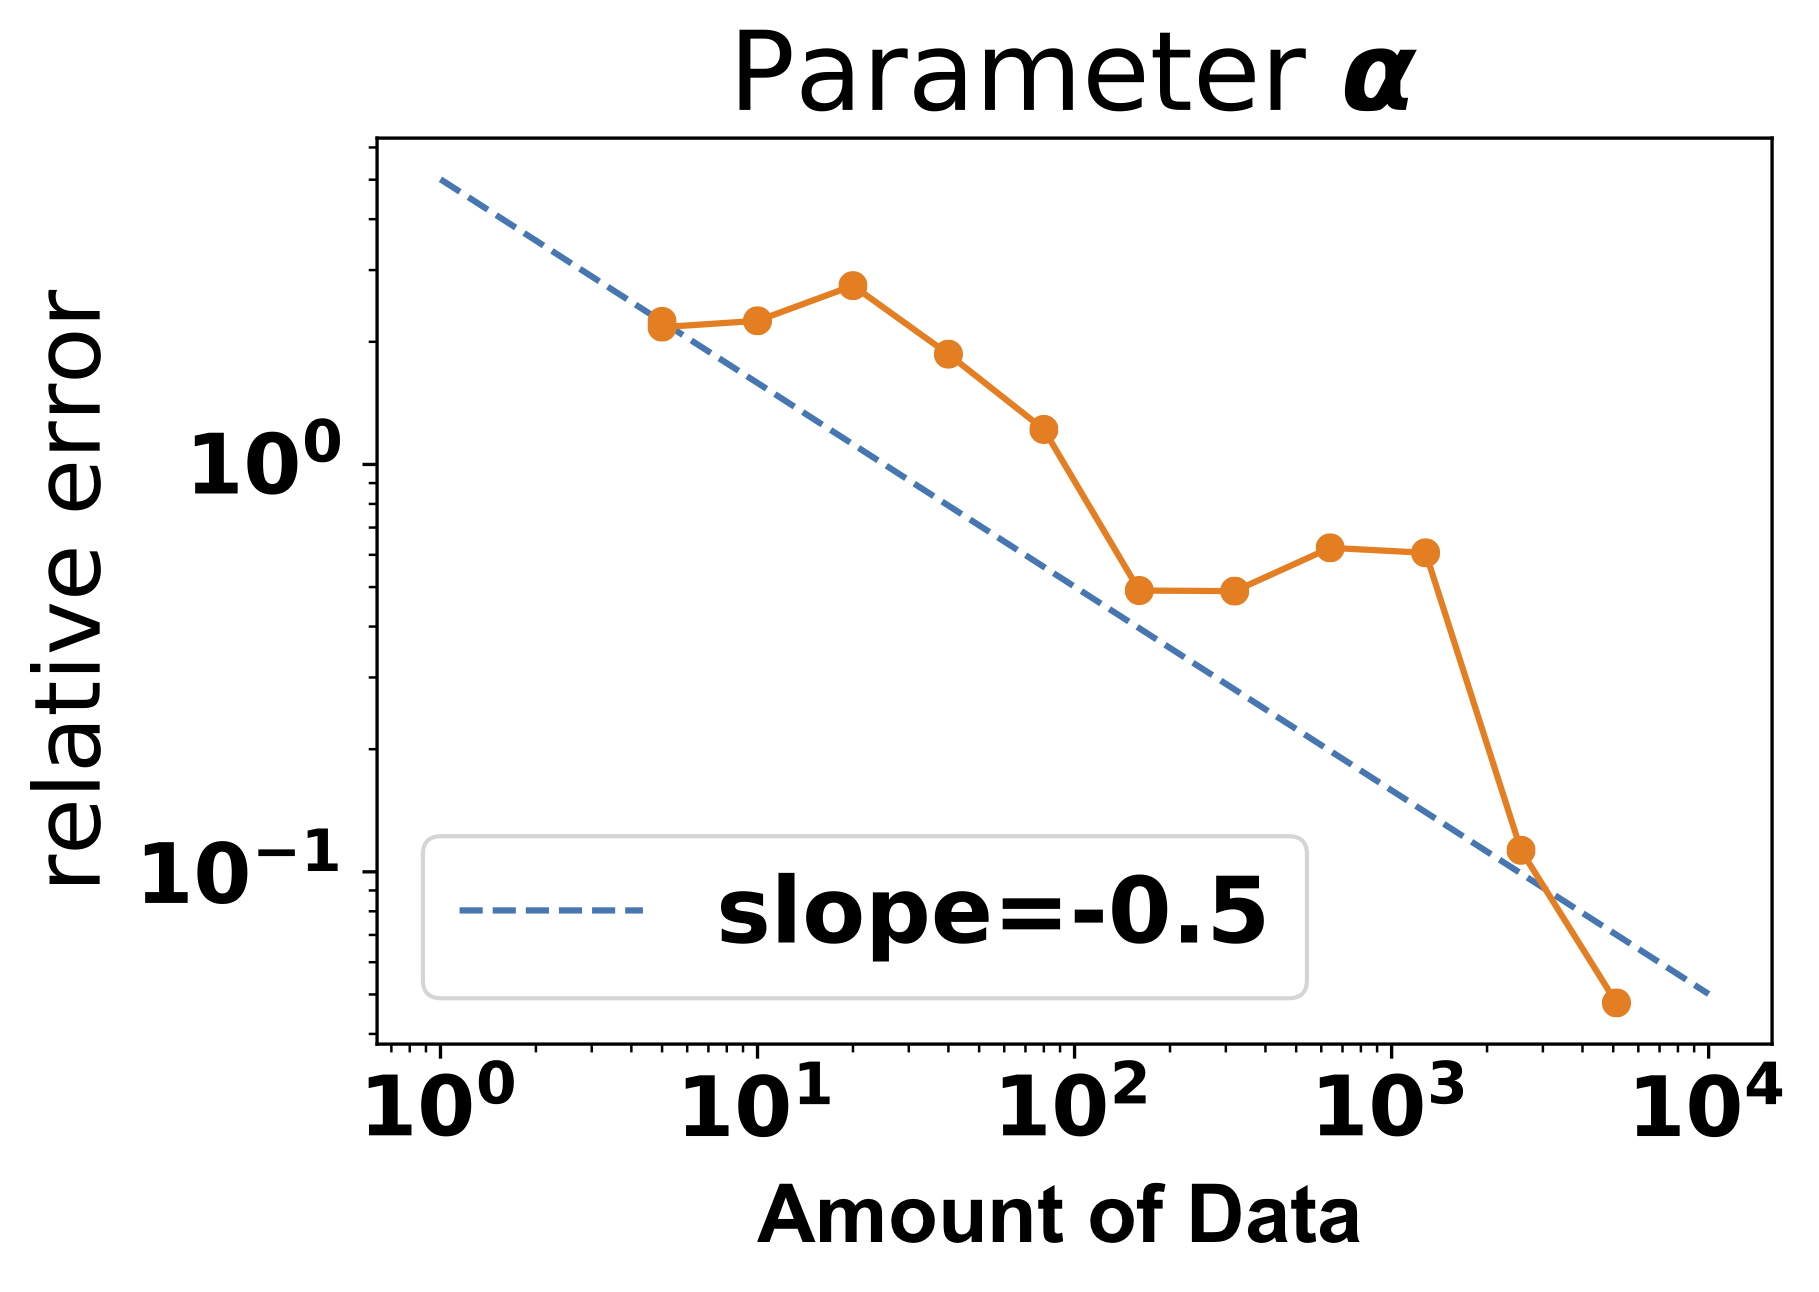
\includegraphics[width=56mm,scale=1]{plots/alpha_conv_beta.png}
  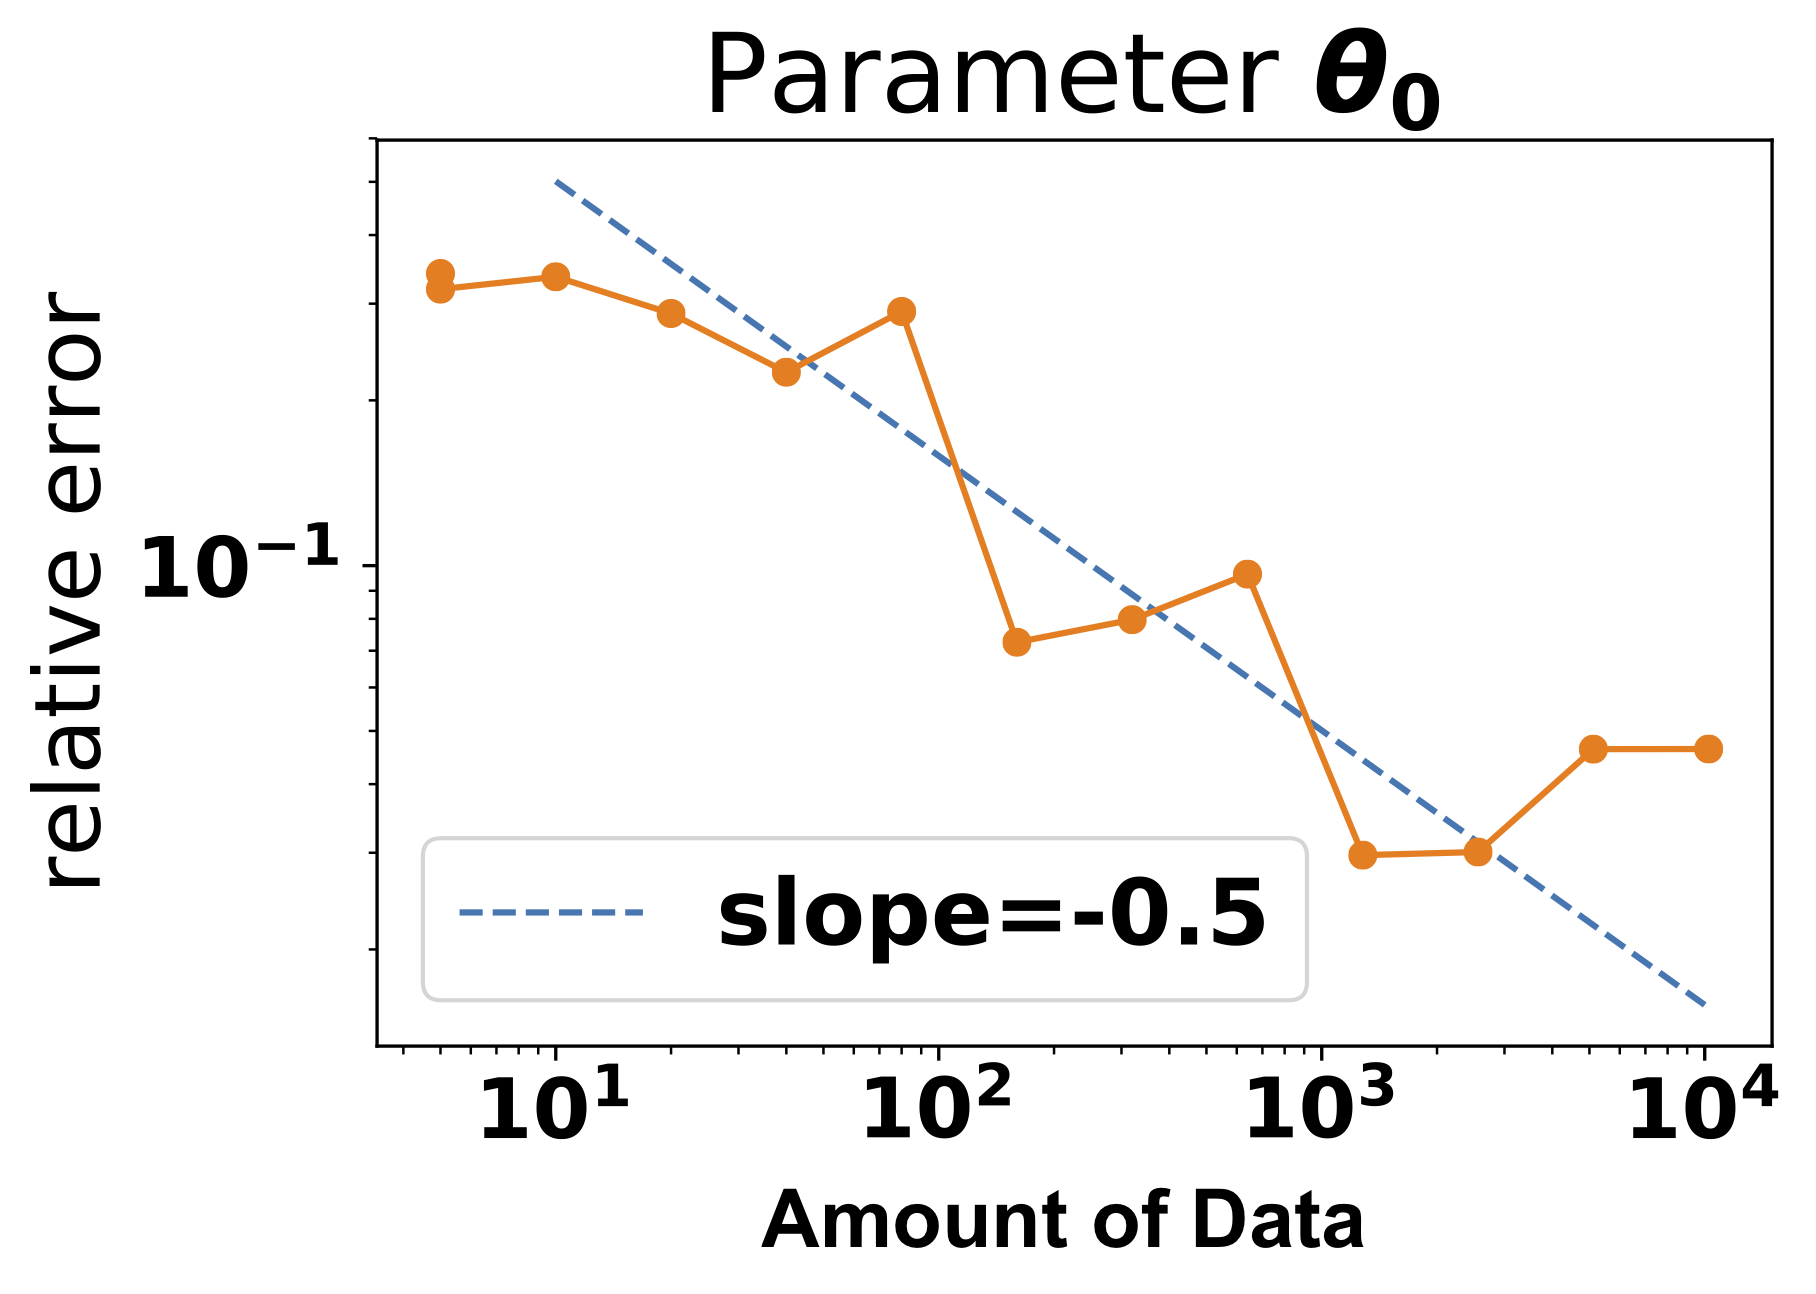
\includegraphics[width=56mm,scale=1]{plots/theta_conv_beta.png}
  \caption{We show self-convergence of our algorithm applied to model $2$. We conlcude that the rate  matches that of of Monte Carlo. Data is from Uruguay pertaining to  year 2018. }
\end{figure}

    \begin{figure}[h]
      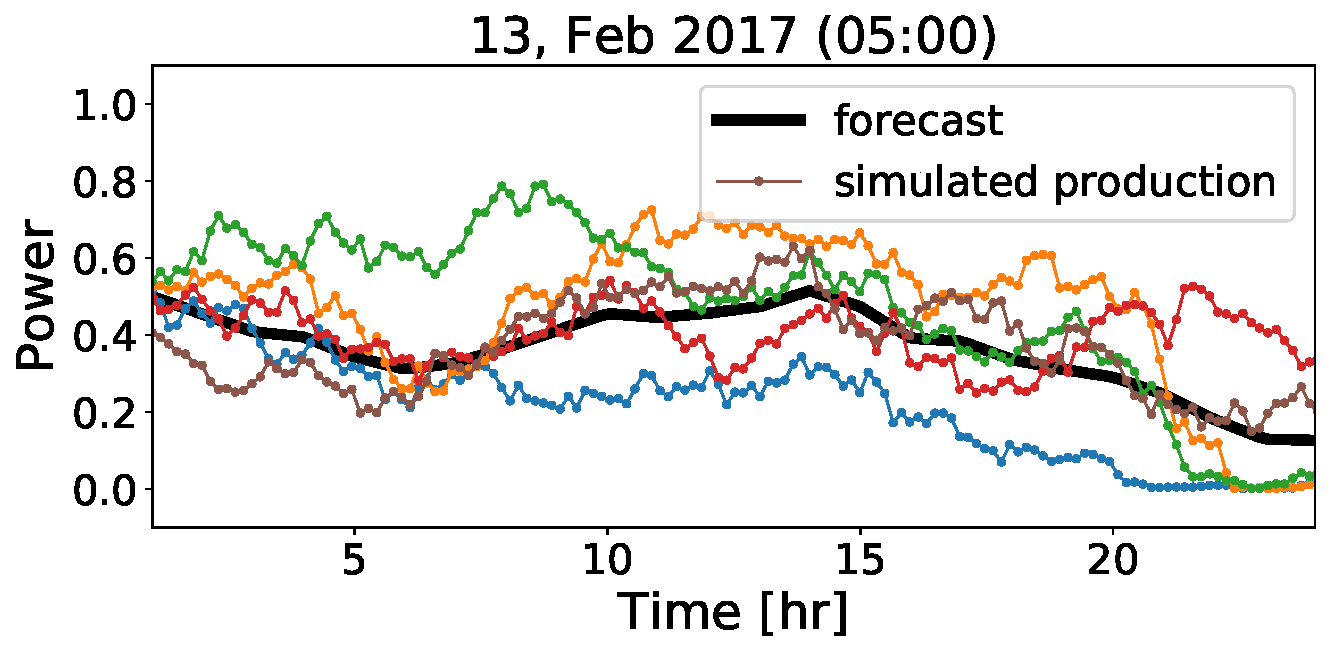
\includegraphics[width=70mm,scale=1]{simulated/24hr/1099.pdf}
      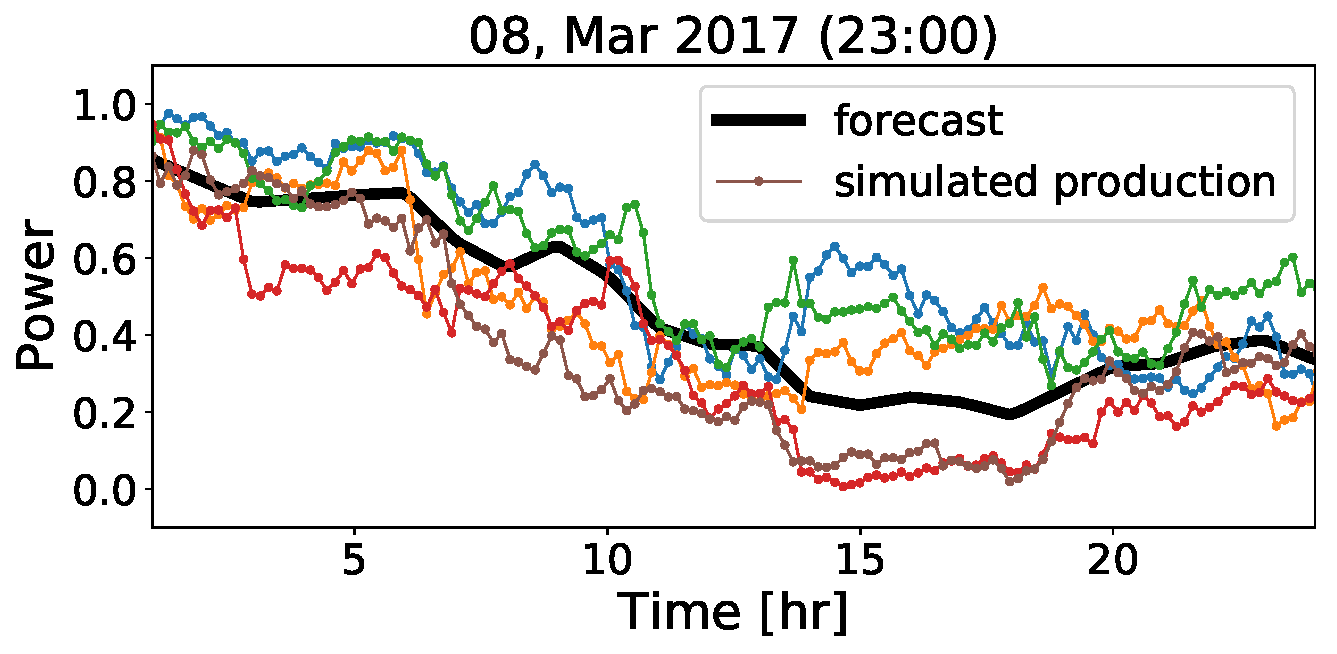
\includegraphics[width=70mm,scale=1]{simulated/24hr/1178.pdf}
      \caption{We simulate following model 2  five possible future wind power production paths using the obtained optimal parameters $(\theta_0, \alpha )=(12,0.3)$. Forecast is from Uruguay pertaining to  year 2018. }
    \end{figure}

    \begin{figure}[h]
      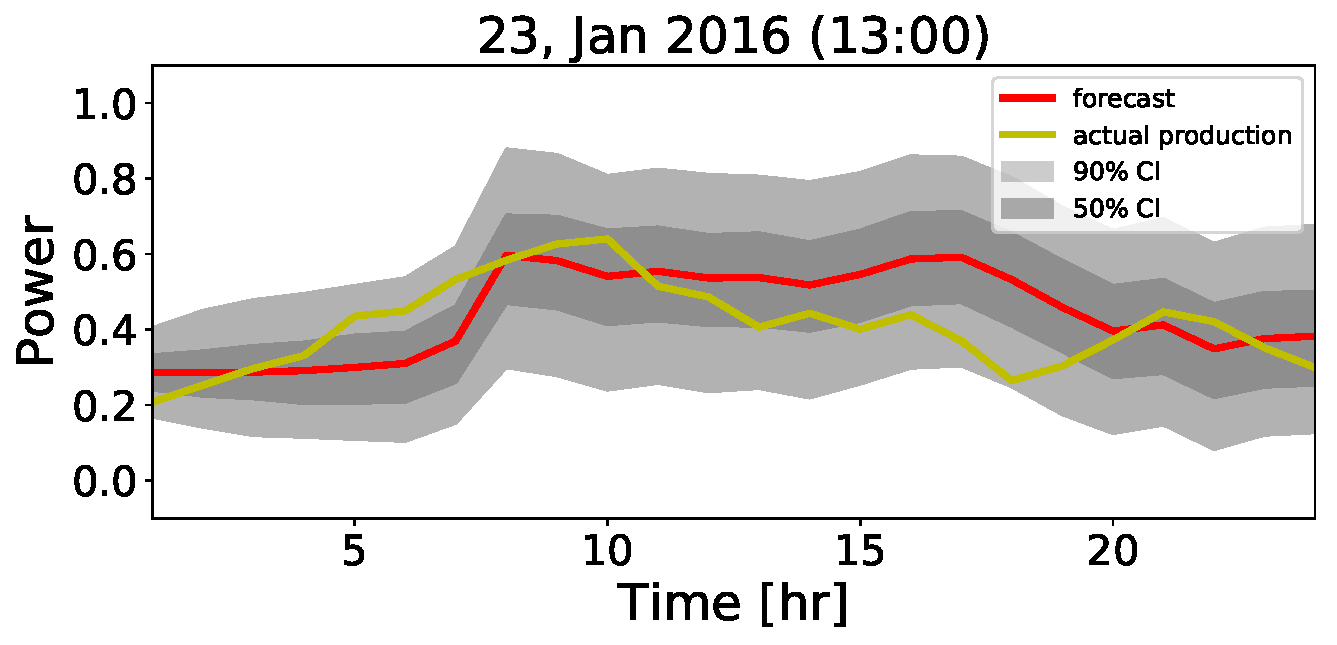
\includegraphics[width=70mm,scale=1]{confidence_intervals/24hr/31.pdf}
      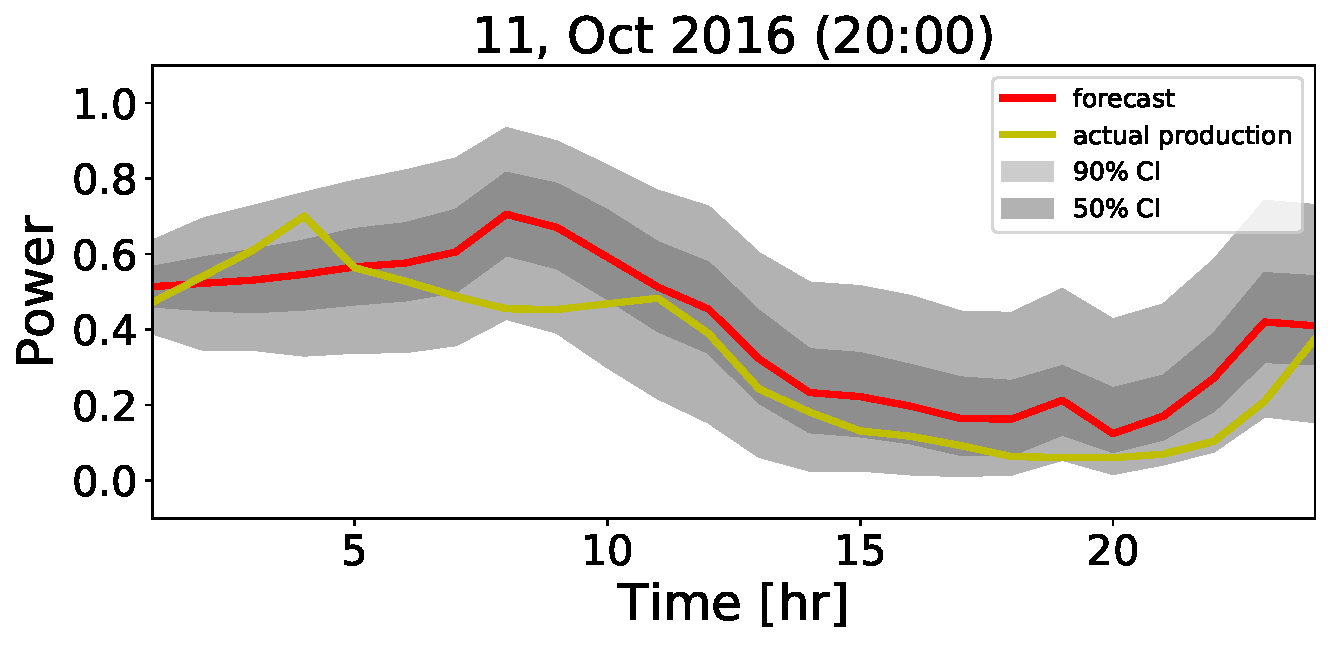
\includegraphics[width=70mm,scale=1]{confidence_intervals/24hr/820.pdf}
       \caption{We obtain confidence intervals following model 2  for future wind power production using the obtained optimal parameters $(\theta_0, \alpha )=(12,0.3)$. Actual production plotted in retrospect. Forecast and data is from Uruguay pertaining to  year 2018. }
    \end{figure}
%---END SECTION 7---

%---BEGIN SECTION 8---
\section{Conclusions} \label{Section_8}

{\color{red} Application: Using this tool, it is possible to iterate over hyper parameters for the wind power forecasting, reaching an optimal forecasting.}

We have proposed a method to produce stochastic wind power forecasts based on parametric SDEs. This method is agnostic of the wind power forecasting technology. Using this method, we were able to simulate future wind power production paths and obtain confidence bands. We conclude that Model 2 is a best-fit model. It features time-derivative tracking of the forecast, time-dependent mean reversion parameter, and a more natural diffusion term. Moreover, the model preserves the asymmetry of wind power forecast errors and their correlation structure.

We were also able to compare two different forecast providers with respect to their real-world performance on the aggregated data set and on specific wind farm sites. Finally, the model paves the way for stochastic optimal control methods enabling optimal decision making under uncertainty.
%---END SECTION 7---

%---REFERENCES---

\nocite{*}
 
%\printbibliography
\printbibliography[keyword={Wind-SDE},title={References}]

\end{document}

